Results here, in past tense.
\comment{Introduce network notation -\Anna}


\subsection{Visualising Sparse Pathways}
    \begin{figure}
        \begin{subfigure}{\linewidth}
            \centering
            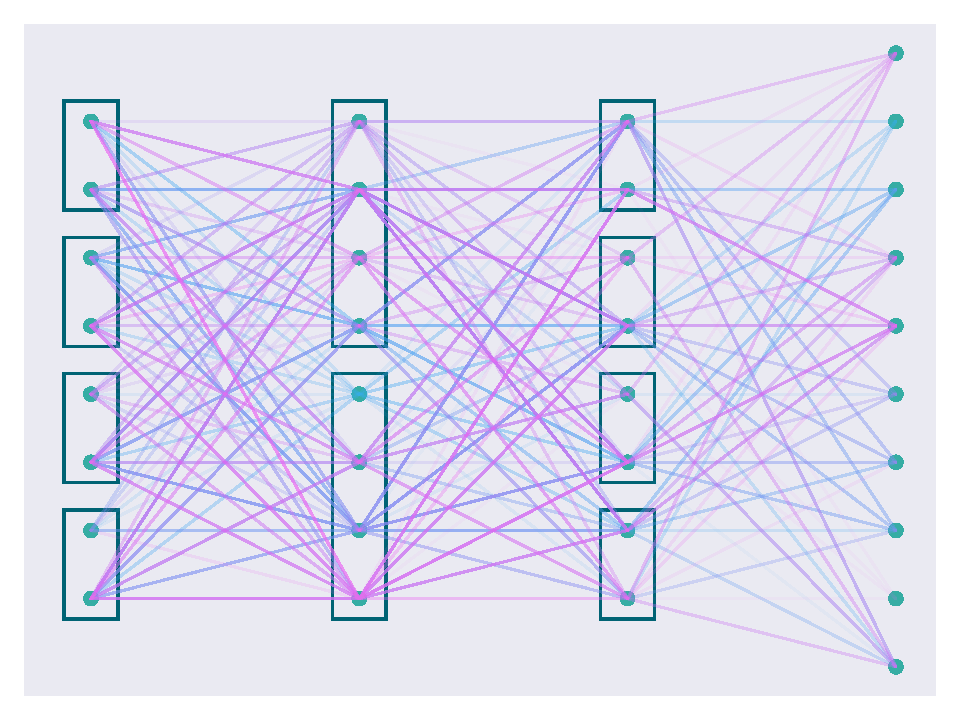
\includegraphics[width=\linewidth]{figs/LWTA_architecture_untrained.pdf}
            \caption{The untrained network predicting validation images of zeros in blue and ones in pink.}
            \label[fig]{res:fig:LWTA_architecture_untrained}
        \end{subfigure}
        \begin{subfigure}{\linewidth}
            \centering
            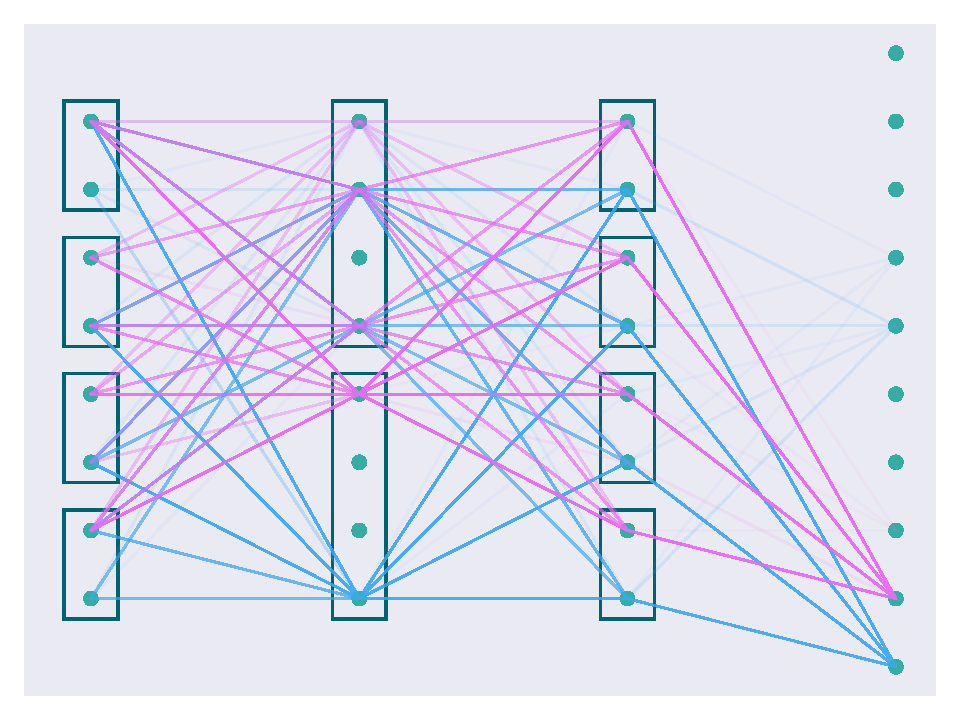
\includegraphics[width=\linewidth]{figs/LWTA_architecture_trained01.pdf}
            \caption{The trained network predicting validation images of zeros in blue and ones in pink.}
            \label[fig]{res:fig:LWTA_architecture_trained01}
        \end{subfigure}
        \begin{subfigure}{\linewidth}
            \centering
            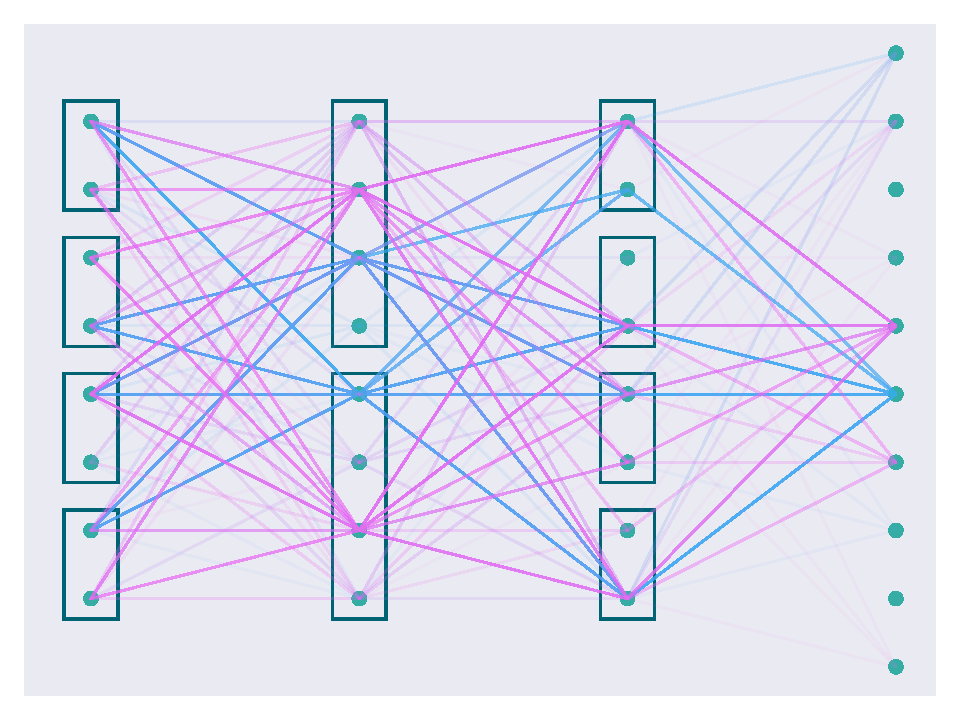
\includegraphics[width=\linewidth]{figs/LWTA_architecture_trained45.pdf}
            \caption{The trained network predicting validation images of fours in blue and fives in pink.}
            \label[fig]{res:fig:LWTA_architecture_trained45}
        \end{subfigure}
        \caption{An illustration of the active pathways as 100 input images belonging to two different classes are passed through a channel-out network. The network was trained on the full training dataset for 26 epochs before stopping early with $p=5$, and had a final validation accuracy of $0.8555$.}
        \label[fig]{res:fig:LWTA_architecture}
    \end{figure}

\subsection{Tuning LWTA Architecture}
    Tuning the architecture of our LWTA networks, we found the maxout network architecture \network{64,64}{32,16} with dropout to do the best on the CIFAR-10 dataset, achieving a test accuracy of 51.57\%. Likewise, the best performing channel-out network architecture was \network{64,16,64}{32,*,32} with L2 penalisation added, achieving a test accuracy of 50.75\%, slightly underperforming maxout. The ordinary ReLU dense network achieved an accuracy of 49.19\% on the test dataset with two layers of 32 nodes. The results are tabulated in \cref{res:tab:networks}.

    \renewcommand{\arraystretch}{2}
    \begin{table}[ht!]
        \centering
        \begin{tabular}{|l|c|c|c|}
        \hline
        & \textbf{Regularisation} & \textbf{Architecture} & \textbf{Accuracy} \\
        \hline
        \rowcolor{mint!20}
        \cellcolor{mint!20} & None & \network{64, 32, 64}{32, 16, 8} & 0.4894 \\ \cline{2-4} 
        \rowcolor{mint!20}
        \cellcolor{mint!20} & Ridge & \network{64, 32}{32, *}  & 0.5094 \\ \cline{2-4} 
        \rowcolor{mint!50}
        \cellcolor{mint!20} & Dropout & \network{64, 64}{32, 16} & 0.5157 \\ \cline{2-4} 
        \rowcolor{mint!20}
        \multirow{-4}{*}{\rotatebox[origin=c]{90}{Maxout}}{\cellcolor{mint!20}} & Both & \network{32, 64}{16, 16} & 0.4938 \\ \hline
        \rowcolor{maroon!20}
        \cellcolor{maroon!20} & None & \network{64, 16, 32}{16, 8, *} & 0.4956 \\ \cline{2-4} 
        \rowcolor{maroon!50}
        \cellcolor{maroon!20} & Ridge & \network{64, 16, 64}{32, *, 32} & 0.5075 \\ \cline{2-4} 
        \rowcolor{maroon!20}
        \cellcolor{maroon!20} & Dropout & \network{32, 16, 64}{16, *, 32} & 0.4826 \\ \cline{2-4} 
        \rowcolor{maroon!20}
        \multirow{-4}{*}{\rotatebox[origin=c]{90}{Channel-Out}}{\cellcolor{maroon!20}} & Both & \network{32, 64}{16, 32} & 0.4917 \\ \hline
        \rowcolor{cyan!20} 
        \cellcolor{cyan!20} & None & \network{32,32}{*,*} & 0.4843 \\ \cline{2-4} 
        \rowcolor{cyan!50} 
        \multirow{-2}{*}{\rotatebox[origin=c]{90}{Dense}}{\cellcolor{cyan!20} } & Ridge & \network{32,32}{*,*} & 0.4919 \\ \hline
        \end{tabular}
        \caption{Table of the best performing network architectures with maxout, channel-out or dense ReLU layers and various combinations of dropout and ridge penalisation added.}
        \label[tab]{res:tab:networks}
    \end{table}
    \renewcommand{\arraystretch}{1}

    \begin{figure}
        \begin{subfigure}{\linewidth}
            \centering
            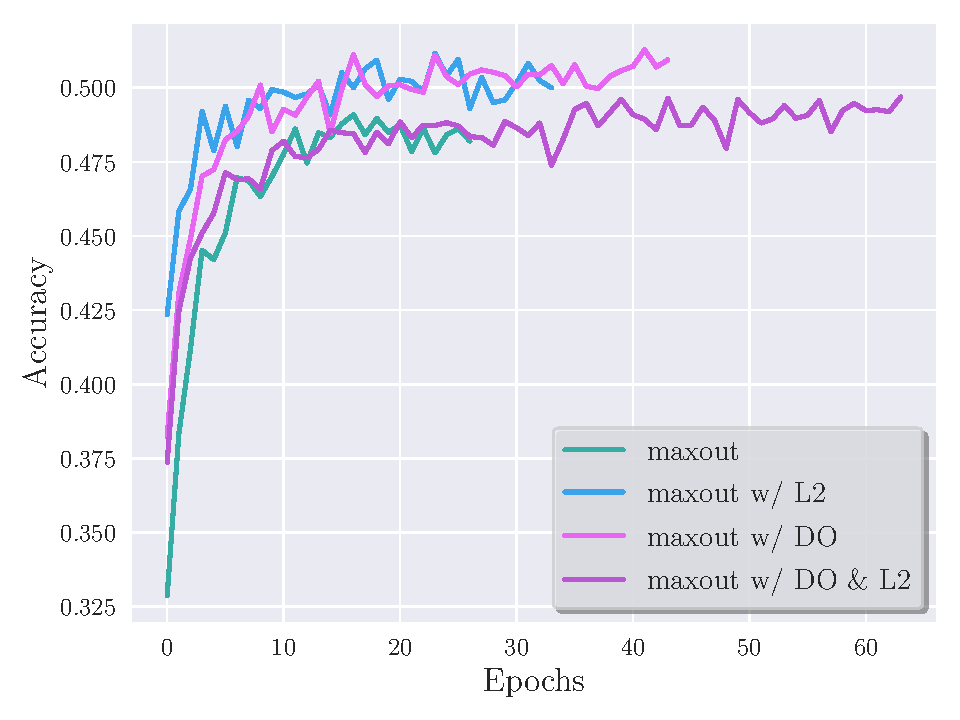
\includegraphics[width=\linewidth]{figs/best_models_maxout.pdf}
            \caption{The test accuracy history of the best performing maxout networks.}
            \label[fig]{res:fig:best_maxout}
        \end{subfigure}
        \begin{subfigure}{\linewidth}
            \centering
            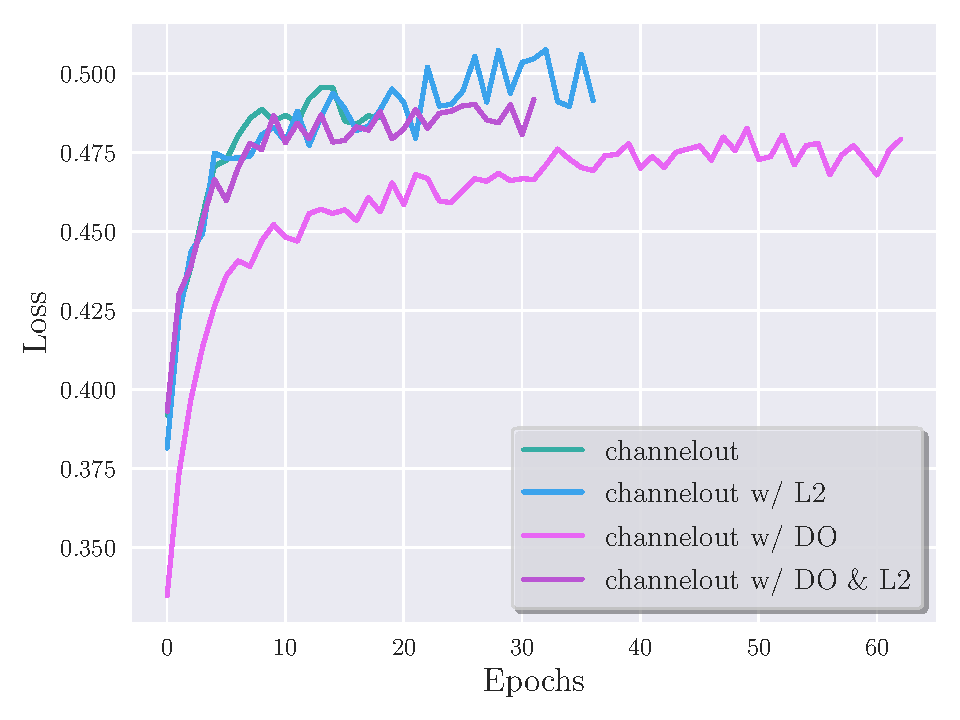
\includegraphics[width=\linewidth]{figs/best_models_channelout.pdf}
            \caption{The test accuracy history of the best performing channel-out networks.}
            \label[fig]{res:fig:best_channelout}
        \end{subfigure}
        \caption{The best performing LWTA models after tuning were trained on the full training dataset and their test accuracy history is plotted here. For the network architecture of the various models see \cref{res:tab:networks}.}
        \label[fig]{res:fig:best_LWTA}
    \end{figure}
    \comment{Discussion note: Comment on the lack of resampling used here. -\Carl}

    \subsubsection{Premier League Dataset}
        \renewcommand{\arraystretch}{2}
        \begin{table}[ht!]
            \centering
            \begin{tabular}{|l|c|c|c|}
            \hline
            & \textbf{Regularisation} & \textbf{Architecture} & \textbf{Accuracy} \\
            \hline
            \rowcolor{mint!20}
            \cellcolor{mint!20} & None & \network{8,16}{*,8} & 0.5403 \\ \cline{2-4} 
            \rowcolor{mint!50}
            \multirow{-2}{*}{\rotatebox[origin=c]{90}{MO}}{\cellcolor{mint!20}} & Both & \network{16, 64}{8, 32} & 0.5806 \\ \hline
            \rowcolor{maroon!50}
            \cellcolor{maroon!20} & None & \network{8,64,16,64}{*,32,*,32} & 0.5484 \\ \cline{2-4} 
            \rowcolor{maroon!20}
            \multirow{-2}{*}{\rotatebox[origin=c]{90}{CO}}{\cellcolor{maroon!20}} & Both & \network{8, 64}{*, 32} & 0.4839 \\ \hline
            \rowcolor{cyan!50} 
            \cellcolor{cyan!20} & None & \network{16,16}{*,*} & 0.5161 \\ \cline{2-4} 
            \rowcolor{cyan!20} 
            \multirow{-2}{*}{\rotatebox[origin=c]{90}{Dense}}{\cellcolor{cyan!20} } & Ridge & \network{16,16}{*,*} & 0.5887 \\ \hline
            \end{tabular}
            \caption{Table of the best performing network architectures with maxout, channel-out or dense ReLU layers and various combinations of dropout and ridge penalisation added.}
            \label[tab]{res:tab:EPL_networks}
        \end{table}
        \renewcommand{\arraystretch}{1}
    
        \begin{figure}
            \centering
            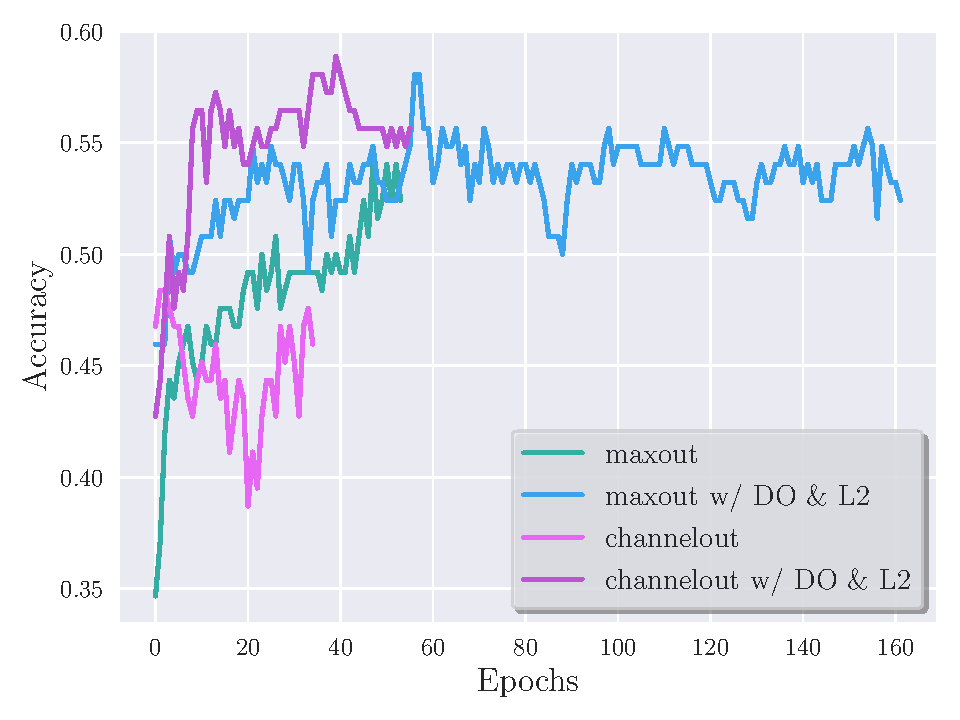
\includegraphics[width=\linewidth]{figs/best_models_EPL.pdf}
            \caption{The history accuracy on the test portion of the EPL dataset of the four best LWTA architectures, with and without regularisation methods added.}
            \label[fig]{res:fig:best_EPL}
        \end{figure}

\subsection{PCA on Premier League data}
    By performing PCA on the Premier League data we found its principal components. The explained variance as a function of principal components is plotted in figure~\ref{res:fig:explained_variance} as both a cumulative sum and histogram bars. As seen from the plot, 42 principal components explains 99 \% of the variance of the original features. \comment{mention something about 99 percent earlier? \Johan}
    \begin{figure}
        \centering
        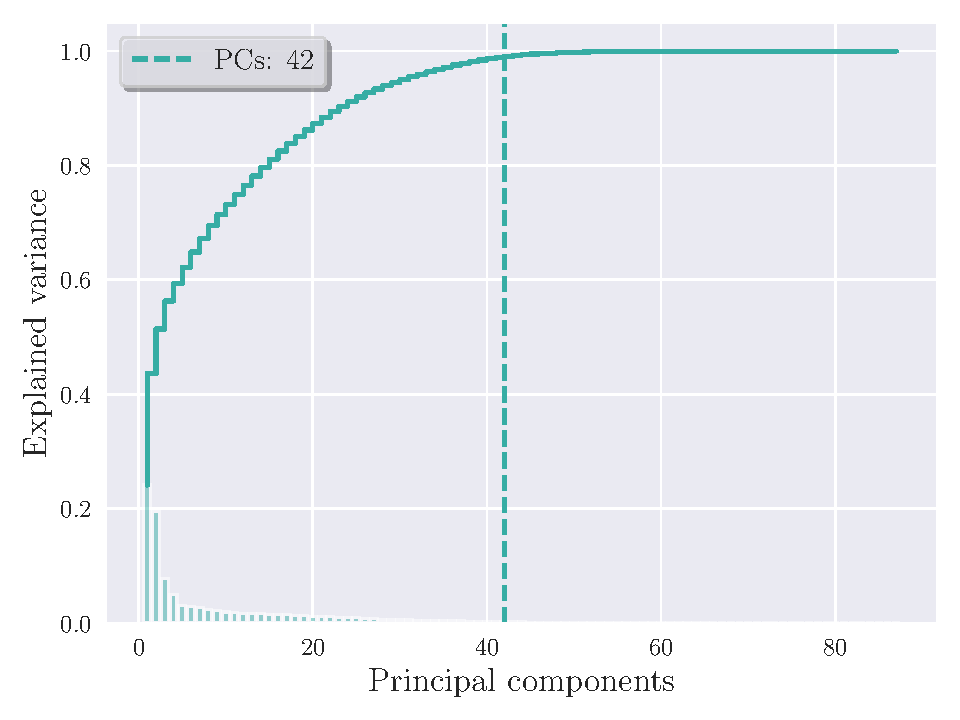
\includegraphics[width=\linewidth]{figs/pca_pl.pdf}
        \caption{Explained variance \comment{writemore and fix plot \Johan}}
        \label[fig]{res:fig:explained_variance}
    \end{figure}

